\documentclass[a4paper, 10pt, twoside]{article}

\usepackage[top=1in, bottom=1in, left=1in, right=1in]{geometry}
\usepackage[utf8]{inputenc}
\usepackage[spanish, es-ucroman, es-noquoting]{babel}
\usepackage{setspace}
\usepackage{fancyhdr}
\usepackage{lastpage}
\usepackage{amsmath}
\usepackage{amsfonts}
\usepackage{amsthm}
\usepackage{verbatim}
\usepackage{graphicx}
\usepackage{float}
\usepackage[noend]{algpseudocode}
\usepackage{enumitem} % Provee macro \setlist
\usepackage[toc, page]{appendix}


%%%%%%%%%% Configuración de Fancyhdr - Inicio %%%%%%%%%%
\pagestyle{fancy}
\thispagestyle{fancy}
\lhead{Trabajo Práctico 2 · Algoritmos y Estructuras de Datos III}
\rhead{Lovisolo · Petaccio · Rossi}
\renewcommand{\footrulewidth}{0.4pt}
\cfoot{\thepage /\pageref{LastPage}}

\fancypagestyle{caratula} {
   \fancyhf{}
   \cfoot{\thepage /\pageref{LastPage}}
   \renewcommand{\headrulewidth}{0pt}
   \renewcommand{\footrulewidth}{0pt}
}
%%%%%%%%%% Configuración de Fancyhdr - Fin %%%%%%%%%%


%%%%%%%%%% Configuración de Algorithmic - Inicio %%%%%%%%%%
% Entorno propio para customizar la presentación del pseudocódigo
\newenvironment{pseudo}[1][]{%
    \vspace{1em}%
    \begin{algorithmic}%
}
{%
    \end{algorithmic}%
    \vspace{1em}%
}

% Valores de verdad
\newcommand{\True}{\textbf{true}}
\newcommand{\False}{\textbf{false}}

% Conectivos lógicos
\newcommand{\PAnd}{\textbf{and} }
\newcommand{\POr}{\textbf{or} }

% Conectivo 'in' para usar así: \ForAll{$foo$ \In $bar$}
\newcommand{\In}{\textbf{in} }

% Conectivo 'to' para usar así: \For{$i = 1$ \In $n$}
\newcommand{\To}{\textbf{to} }

% Control de flujo
\newcommand{\Break}{\State \textbf{break}}
\newcommand{\PReturn}{\State \textbf{return} }

% Complejidades
\newcommand{\Ode}[1]{\hfill $O(#1)$}
%%%%%%%%%% Configuración de Algorithmic - Fin %%%%%%%%%%


%%%%%%%%%% Miscelánea - Inicio %%%%%%%%%%
% Evita que el documento se estire verticalmente para ocupar el espacio vacío
% en cada página.
\raggedbottom

% Deshabilita sangría en la primer línea de un párrafo.
\setlength{\parindent}{0em}

% Separación entre párrafos.
\setlength{\parskip}{0.5em}

% Separación entre elementos de listas.
\setlist{itemsep=0.5em}

% Asigna la traducción de la palabra 'Appendices'.
\renewcommand{\appendixtocname}{Apéndices}
\renewcommand{\appendixpagename}{Apéndices}
%%%%%%%%%% Miscelánea - Fin %%%%%%%%%%


%%%%%%%%%% Gráficos - Inicio %%%%%%%%%%
% Macro para incluir tres gráficos (dentro de una figura) de manera que
% entren todos en una sola página.
\newcommand{\tresgraficos}[3]{
    \newcommand{\separacion}{-2.2em}
    \vspace{\separacion}
    \include{#1}
    \vspace{\separacion}
    \include{#2}
    \vspace{\separacion}
    \include{#3}
}

% Macro para incluir dos gráficos (dentro de una figura) de manera que
% entren todos en una sola página.
\newcommand{\dosgraficos}[2]{
    \newcommand{\separacion}{-2.2em}
    \vspace{\separacion}
    \include{#1}
    \vspace{\separacion}
    \include{#2}
}
%%%%%%%%%% Gráficos - Fin %%%%%%%%%%


\begin{document}


%%%%%%%%%%%%%%%%%%%%%%%%%%%%%%%%%%%%%%%%%%%%%%%%%%%%%%%%%%%%%%%%%%%%%%%%%%%%%%%
%% Carátula                                                                  %%
%%%%%%%%%%%%%%%%%%%%%%%%%%%%%%%%%%%%%%%%%%%%%%%%%%%%%%%%%%%%%%%%%%%%%%%%%%%%%%%


\thispagestyle{caratula}

\begin{center}


\includegraphics[height=2cm]{DC.png} 
\hfill

\includegraphics[height=2cm]{UBA.jpg} 

\vspace{2cm}

Departamento de Computación,\\
Facultad de Ciencias Exactas y Naturales,\\
Universidad de Buenos Aires

\vspace{4cm}

\begin{Huge}
Trabajo Práctico 2
\end{Huge}

\vspace{0.5cm}

\begin{Large}
Algoritmos y Estructuras de Datos III
\end{Large}

\vspace{1cm}

Segundo Cuatrimestre de 2013

\vspace{4cm}

\begin{tabular}{|c|c|c|}
\hline
Apellido y Nombre & LU & E-mail\\
\hline
Leandro Lovisolo      & 645/11 & leandro@leandro.me\\
Lautaro José Petaccio & 443/11 & lausuper@gmail.com\\
Lucas Rossi           & 705/11 & lucasrossi20@gmail.com\\
\hline
\end{tabular}

\end{center}

\newpage


%%%%%%%%%%%%%%%%%%%%%%%%%%%%%%%%%%%%%%%%%%%%%%%%%%%%%%%%%%%%%%%%%%%%%%%%%%%%%%%
%% Índice                                                                    %%
%%%%%%%%%%%%%%%%%%%%%%%%%%%%%%%%%%%%%%%%%%%%%%%%%%%%%%%%%%%%%%%%%%%%%%%%%%%%%%%


\tableofcontents

\newpage


%%%%%%%%%%%%%%%%%%%%%%%%%%%%%%%%%%%%%%%%%%%%%%%%%%%%%%%%%%%%%%%%%%%%%%%%%%%%%%%
%% Introducción                                                              %%
%%%%%%%%%%%%%%%%%%%%%%%%%%%%%%%%%%%%%%%%%%%%%%%%%%%%%%%%%%%%%%%%%%%%%%%%%%%%%%%


\section{Introducción}

En el presente trabajo estudiamos tres problemas algorítmicos, proponemos soluciones para los mismos respetando sus requerimientos de complejidad temporal y analizamos empíricamente los tiempos de ejecución de sus implementaciones en lenguaje C++.

La motivación de este trabajo es comparar las cotas temporales obtenidas del análisis teórico con las mediciones de tiempos de ejecución y extraer conclusiones de esta experimentación.

Sin más, presentamos los problemas estudiados a continuación.


%%%%%%%%%%%%%%%%%%%%%%%%%%%%%%%%%%%%%%%%%%%%%%%%%%%%%%%%%%%%%%%%%%%%%%%%%%%%%%%
%% Problema 1: Impresiones ordenadas                                         %%
%%%%%%%%%%%%%%%%%%%%%%%%%%%%%%%%%%%%%%%%%%%%%%%%%%%%%%%%%%%%%%%%%%%%%%%%%%%%%%%


\newpage

\section{Problema 1: Impresiones ordenadas}

A una imprenta se le encarga una serie de trabajos $t_1, \cdots, t_n$ que deben ser realizados en el orden dado, sin excepción.

La imprenta posee dos impresoras. Cada impresora debe prepararse adecuadamente antes de realizar un trabajo (por ejemplo, se les debe cargar la tinta y el papel correcto.)

Esta preparación tiene un costo asociado que depende del último trabajo realizado en esa impresora y del trabajo para el cual se la desea preparar. Preparar una impresora para realizar el trabajo $t_j$ luego de haber realizado el trabajo $t_i$ tiene costo $c_{ij}$, con $i < j$.

Preparar una impresora para el $i$-ésimo trabajo cuando ésta aún no realizó ningún trabajo también tiene un costo asociado, al que denotaremos $c_{0i}$.

Se nos pide escribir un algoritmo que, dada una cantidad de trabajos $n$ y los costos de preparación $c_{ij}$ correspondientes, determine en qué máquina realizar cada trabajo de manera que la suma de los costos de preparación sea mínima, y devuelva el costo hallado y la cola de trabajos de alguna de las impresoras. El algoritmo debe tener una cota de complejidad temporal de peor caso $O(n^2)$.

\textbf{Ejemplos del problema y sus soluciones:}

\textbf{Entrada:} $n = 1$, $c_{0, 1} = 1$. \\
\textbf{Salida:} $\{ 1 \}$ (costo total: 1)

\textbf{Entrada:} $n = 3$, $c_{0, 1} = 1$, $c_{0, 2} = 2$, $c_{0, 3} = 3$, 
                           $c_{1, 2} = 4$, $c_{1, 3} = 5$, $c_{2, 3} = 6$. \\
\textbf{Salida:} $\{ 1, 2 \}$ (costo total: 8)


\subsection{Solución}

Resolvemos este problema aplicando la técnica de programación dinámica.

Representamos los últimos trabajos realizados en cada máquina con el par $(i, j)$. Si una de las máquinas aún no realizó ningún trabajo, ponemos un $0$ en su respectivo componente del par. Para simplificar el razonamiento, asumimos de aquí en adelante que $i < j$.

Sea $C(i, j)$ la función que devuelve el costo mínimo de realizar \textbf{los trabajos restantes} cuando los últimos trabajos hechos en cada impresora fueron $t_i$ y $t_j$.

Por ejemplo, para el lote de trabajos $t_1, \cdots, t_6$, vale que $C(1, 3)$ es el costo mínimo de realizar los trabajos $t_4$, $t_5$ y $t_6$ cuando los últimos trabajos realizados en cada impresora fueron $t_1$ y $t_3$.

Podemos definir $C(i, j)$ recursivamente de la siguiente manera, respetando siempre que $i < j$:

$$
C(i, j) =
\left\{
  \begin{array}{ll}
    min\{ C(i, j + 1) + c_{j, j + 1}, \; C(j, j + 1) + c_{i, j + 1} \} & \mbox{si } j < n \\
    0                                                                  & \mbox{si } j = n \\
    \infty                                                             & \mbox{si } i \geq j \mbox{ (caso ińválido)}
  \end{array}
\right.
$$

Si $j < n$, comparamos el costo de realizar $t_{j + 1}$ en cada de las impresoras y nos quedamos con el menor. Si $j = n$, quiere decir que el último trabajo realizado fue $t_n$, es decir que no quedan más trabajos por hacer, entonces el costo de realizar los trabajos restantes es cero.

Lo que nos interesa entonces es hallar $C(0, 0)$, es decir, el costo mínimo de realizar el lote de trabajos $t_1, \cdots, t_n$ cuando las máquinas aún no realizaron ningún trabajo.

El algoritmo a continuación computa cada $C(i, j)$ de manera \textit{bottom-up}, memoriza los resultados en un arreglo $dp$ y luego construye una solución recorriendo este arreglo.


\subsubsection{Pseudocódigo}

Sean $n$ la cantidad de trabajos a realizar, $dp$ un arreglo de enteros no negativos de dimensión $(n + 1) \times (n + 1)$ y $c$ otro arreglo de mismo tipo y dimensión que contiene los costos de preparación de las máquinas\footnote{Notar que no todas las coordenadas de $c$ son válidas; por ejemplo $c[2][1] = c_{2,1}$ no representa un costo válido pues el trabajo 1 nunca puede realizarse después del trabajo 2.}, tal que $c[i][j] = c_{ij}$.


\begin{pseudo}
  \Procedure{Impresiones-Ordenadas}{$n, c$}
    \State $dp \leftarrow $ arreglo de enteros de dimensión $(n + 1) \times (n + 1)$,
           inicializado en 0                                                              \Ode{n^2}
    \For{$j \leftarrow n - 1$ \To $0$} \Comment{Computamos $dp$}
      \For{$i \leftarrow 0$ \To $n - 1$}
        \If{$i = 0$ \PAnd $j = 0$} \Comment{El costo que queremos hallar}
          \State $dp[0][0] \leftarrow dp[0][1] + c[0][1]$                                 \Ode{1}
          \Break
        \EndIf

        \If{$i = j$} \Comment{Estado inválido}
          \Break
        \EndIf

        \State $dp[i][j] \leftarrow \textsc{min}(dp[i][j + 1] + c[j][j + 1],$ \Comment{Caso general}
        \State \phantom{$dp[i][j] \leftarrow \textsc{min}($}$dp[j][j + 1] + c[i][j + 1])$ \Ode{1}
      \EndFor
    \EndFor

    \State $t \leftarrow \{ 1 \}$ \Comment{Cola de trabajos de una de las impresoras}
    \State $i \leftarrow 0$, $j \leftarrow 1$ \Comment{Comenzamos desde el estado $(0, 1)$}

    \While{$j < n$} \Comment{Recorremos el arreglo $dp$ y construimos $t$}
      \If{$dp[i][j] = dp[i][j + 1] + c[j][j + 1]$} \Comment{Avanzamos de $(i, j)$ a $(i, j + 1)$}
        \If{$\textsc{último}(t) = j$}                                                     \Ode{1}
          \State $t \leftarrow t \cup \{j + 1 \}$                                         \Ode{1}
        \EndIf
        \State $j \leftarrow j + 1$
      \Else \Comment{Avanzamos de $(i, j)$ a $(j, j + 1)$}
        \If{$\textsc{último}(t) = i$}                                                     \Ode{1}
          \State $t \leftarrow t \cup \{j + 1 \}$                                         \Ode{1}
        \EndIf
        \State $i \leftarrow j$
        \State $j \leftarrow j + 1$    
      \EndIf
    \EndWhile

    \PReturn $t$
  \EndProcedure
\end{pseudo}


\subsection{Complejidad}

El algoritmo inicializa el arreglo $dp$ con costo $O(n^2)$, luego computa cada coordenada válida de $dp$ en dos ciclos anidados con cantidad de iteraciones $O(n^2)$ y finalmente construye una solución a partir de $dp$ en un ciclo de $O(n)$ iteraciones.

La complejidad total es $O(n^2) + O(n^2) + O(n) = O(n^2)$.


\subsection{Correctitud}

A continuación vemos que el problema exhibe subestructura óptima y solapamiento de subproblemas, lo cual nos permite aplicar la técnica de programación dinámica.

Luego verificamos que se computa correctamente el costo mínimo de cada subproblema, y que se construye correctamente una solución óptima concreta a partir de los valores memoizados.


\subsubsection{Subestructura óptima}

Consideremos el problema $(i, j)$. Los últimos trabajos realizados por cada impresora son $t_i$ y $t_j$, con $i < j$. Nos interesa hallar $C(i, j)$, es decir el costo mínimo de realizar los trabajos $t_{j + 1}, \cdots, t_n$. Tenemos dos opciones: realizar $t_{j + 1}$ en la primera impresora o bien en la segunda.

Supongamos que el costo mínimo se obtiene realizando $t_{j + 1}$ en la segunda impresora. Entonces vale que $C(i, j) = c_{j, j + 1} + C(i, j + 1)$.

Supongamos ahora que existe otra forma más barata de resolver el subproblema $(i, j + 1)$; llamémosla $C'(i, j + 1)$. Entonces vale $C'(i, j + 1) < C(i, j + 1)$.

Sea $C'(i, j)$ el costo de resolver el problema $(i, j)$ utilizando esta nueva solución al subproblema $(i, j + 1)$. Entonces vale $C'(i, j) = c_{j, j + 1} + C'(i, j + 1) < c_{j, j + 1} + C(i, j + 1) = C(i, j)$, lo cual es absurdo pues $C(i, j)$ es el costo mínimo de resolver el problema $(i, j)$ y no existe otra solución con costo menor.

Luego, el problema exhibe subestructura óptima.


\subsubsection{Solapamiento de subproblemas}

Consideremos el problema $(0, 2)$. El siguiente trabajo a encolar es $t_3$, por lo que para determinar $C(0, 2)$ necesitamos conocer los subproblemas $C(2, 3)$ y $C(0, 3)$.

Consideremos ahora el problema $(1, 2)$. El siguiente trabajo a encolar también es $t_3$, por lo que para determinar $C(1, 2)$ necesitamos conocer los subproblemas $C(2, 3)$ y $C(1, 3)$.

Notemos que los problemas $(0, 2)$ y $(1, 2)$ ambos comparten el subproblema $(2, 3)$.

Luego, el problema exhibe solapamiento de subproblemas.


\subsubsection{Costo mínimo de cada subproblema}

Veamos la sección del algoritmo dedicada a computar el costo mínimo de cada subproblema.

\begin{pseudo}
  \State $dp \leftarrow $ arreglo de enteros de dimensión $(n + 1) \times (n + 1)$,
           inicializado en 0  
  \For{$j \leftarrow n - 1$ \To $0$}
    \For{$i \leftarrow 0$ \To $n - 1$}
      \State \ldots computar $dp[i][j]$
    \EndFor
  \EndFor
\end{pseudo}

El ciclo anidado computa $C(i, j)$ y guarda el valor hallado en $dp[i][j]$. Para computar $C(i, j)$ es necesario computar $C(i, j + 1)$ y $C(j, j + 1)$. Como el algoritmo resuelve el problema de manera \textit{bottom-up}, estos valores deben haber sido computados previamente y guardados en $dp[i][j + 1]$ y $dp[j][j + 1]$, respectivamente. Veamos que esto se cumple.

\textbf{Caso base:} Los costos $C(0, n), \cdots, C(n - 1, n)$ siempre tienen valor 0, pues representan el costo de realizar los trabajos restantes luego de finalizar $t_n$, es decir, el conjunto vacío. Como $dp$ se inicializa en 0, cada entrada en $dp$ correspondiente a los valores $C(0, n), \cdots, C(n - 1, n)$ tiene el valor correcto, y dado que el ciclo exterior asigna a $j$ los valores en el rango $n - 1, \cdots, 0$, nunca se vuelven a escribir las entradas $dp[0][n], \cdots, dp[n - 1][n]$.

\textbf{Caso general:} La iteración computa $C(i, j)$. Veamos que disponemos de los valores de $C(i, j + 1)$ y $C(j, j + 1)$. El ciclo exterior asigna a $j$ los valores en el rango $n - 1, \cdots, 0$. Entonces antes de procesar la columna $j$, primero se procesa la columna $j + 1$. Es cierto que se computa $C(i, j + 1)$ al procesarse la columna $j + 1$, pues el ciclo interior recorre los valores de $i$ en el rango $0, \cdots, j$ y vale que $i < j$. De igual manera, es cierto que se computa $C(j, j + 1)$ al procesarse la columna $j + 1$, pues el ciclo interior recorre los valores de $i$ en el rango $0, \cdots, j$ y vale que $i = j$. Luego, $dp[i][j + 1]$ y $dp[j][j + 1]$ guardan los valores necesarios para computar $C(i, j)$.

Vimos que los subproblemas se computan en el orden correcto. Veamos ahora que los valores $dp[i][j]$ hallados respetan la definición de $C(i, j)$:

$$
C(i, j) =
\left\{
  \begin{array}{ll}
    min\{ C(i, j + 1) + c_{j, j + 1}, \; C(j, j + 1) + c_{i, j + 1} \} & \mbox{si } j < n \\
    0                                                                  & \mbox{si } j = n \\
    \infty                                                             & \mbox{si } i \geq j \mbox{ (caso ińválido)}
  \end{array}
\right.
$$

Para el problema general, el algoritmo asigna el valor $dp[0][0] \leftarrow dp[0][1] + c[0][1]$. Entonces es cierto que $dp[0][0] = min\{ C(0, 1) + c_{0, 1}, \; C(0, 1) + c_{0, 1} \}$.

Para los subproblemas, el algoritmo asigna el valor $dp[i][j] \leftarrow \textsc{min}(dp[i][j + 1] + c[j][j + 1], \; dp[j][j + 1] + c[i][j + 1])$. Entonces es cierto que $dp[i][j] =min\{ C(i, j + 1) + c_{j, j + 1}, \; C(j, j + 1) + c_{i, j + 1} \}$.

Para los casos base, el algoritmo inicializa $dp[0][n], \cdots, dp[n - 1][n]$ en 0, entonces se condice con la segunda rama de $C$ ($j = n$).

Luego, el costo mínimo de cada subproblema se computa correctamente.


\subsubsection{Construcción de una solución óptima}

El problema pide devolver la cola de trabajos de cualquiera de las impresoras. El algoritmo propuesto siempre devuelve la cola correspondiente a la impresora en la que se realizó el trabajo $t_1$. Veamos qué sucede con los trabajos $t_2, \cdots, t_n$.

El costo de la solución óptima $C(0, 0)$ está memoizado en $dp[0][0]$ y depende únicamente de $C(0, 1)$, que está memoizado en $dp[0][1]$. A su vez, el valor de $C(0, 1)$ depende de $C(0, 2)$ y $C(1, 2)$, memoizados en $dp[0][2]$ y $dp[1][2]$, respectivamente. Queremos saber en qué impresora se realiza el trabajo $t_2$.

Si $t_2$ se realiza en la misma impresora que $t_1$ entonces vale que $dp[0][1] = dp[0][2] + c[1][2]$. Por el contrario, si $t_2$ se realiza en la otra impresora, que hasta el momento no realizó ningún trabajo, entonces vale que $dp[0][1] = dp[1][2] + c[0][2]$. Entonces la cola de trabajos devuelta por el algoritmo comenzará con $\{ t_1, t_2 \}$ si $dp[0][1] = dp[0][2] + c[1][2]$ ó $\{ t_1 \}$ si $dp[0][1] = dp[1][2] + c[0][2]$.

Consideremos ahora un subproblema cualquiera $(i, j)$. Su costo mínimo $C(i, j)$ está memoizado en $dp[i][j]$ y éste depende de $C(i, j + 1)$ y $C(j, j + 1)$, memoizados en $dp[i][j + 1]$ y $dp[j][j + 1]$, respectivamente.  Queremos saber en qué impresora se realiza el trabajo $t_{j + 1}$.

Si $t_{j + 1}$ se encola en la misma impresora que $t_j$ entonces vale que $dp[i][j] = dp[i][j + 1] + c[j][j + 1]$. Si en cambio $t_{j + 1}$ se encola en la misma impresora que $t_i$, entonces vale que $dp[i][j] = dp[j][j + 1] + c[i][j + 1]$.

Con esto último ya estamos en condiciones de construir la cola de trabajos devuelta por el algoritmo: si el último trabajo en dicha cola coincide con el último trabajo de la impresora en la que se encoló $t_{j + 1}$, lo agregamos al final de la cola devuelta por el algoritmo.

El pseudocódigo refleja lo explicado recién: primero inicializa la cola de trabajos $t$ agregando el primer trabajo: $t \leftarrow \{ 1 \}$. Luego comienza un ciclo con $i = 0$ y $j = 1$, en el que evalua $dp[i][j]$ para determinar en qué impresora se encoló $t_{j + 1}$, agrega este trabajo a $t$ si $\textsc{último}(t)$ coincide con el último trabajo de la impresora en la que se encoló $t_{j + 1}$ y actualiza $i$ y $j$ según corresponda, hasta llegar a un caso base ($j = n$).


\subsection{Instancias del problema para verificar la correctitud del algoritmo}

\textbf{Caso borde:} Un sólo trabajo.

\textbf{Entrada:} $n = 1$, $c_{0, 1} = 1$. \\
\textbf{Salida:} $\{ 1 \}$ (costo total: 1)
\\

\textbf{Caso borde:} Todos los trabajos en la misma impresora.

\textbf{Entrada:} $n = 3$, $c_{0, 1} = 1$, $c_{0, 2} = 10$, $c_{0, 3} = 10$, 
                           $c_{1, 2} = 1$, $c_{1, 3} = 10$, $c_{2, 3} = 1$. \\
\textbf{Salida:} $\{ 1, 2, 3 \}$ (costo total: 3)
\\

\textbf{Caso general:} Trabajos repartidos entre ambas impresoras.

\textbf{Entrada:} $n = 3$, $c_{0, 1} = 1$, $c_{0, 2} = 2$, $c_{0, 3} = 3$, 
                           $c_{1, 2} = 4$, $c_{1, 3} = 5$, $c_{2, 3} = 6$. \\
\textbf{Salida:} $\{ 1, 2 \}$ (costo total: 8)


\subsection{Experimentos computacionales}

Realizamos dos conjuntos de experimentos: caso general e instancias aleatorias.

Para el caso general, medimos el tiempo de ejecución para cantidad de trabajos $n$ en el rango $1, \cdots, 1000$ y asignamos los costos de preparación $c_{ij}$ de forma creciente. Por ejemplo, para $n = 3$ estos costos serían $c_{0, 1} = 1$, $c_{0, 2} = 2$, $c_{0, 3} = 3$, $c_{1, 2} = 4$, $c_{1, 3} = 5$, $c_{2, 3} = 6$.

Los experimentos sobre instancias aleatorias se realizan de la misma manera, con la diferencia que los costos $c_{ij}$ se toman de un generador de números pseudoaleatorios.

\newpage


\subsubsection{Caso general}

\begin{figure}[H]
  \centering
  \tresgraficos{problema1-caso-general}
               {problema1-caso-general-n}
               {problema1-caso-general-n2}
  \caption{Caso general}
\end{figure}


\subsubsection{Instancias aleatorias}

\begin{figure}[H]
  \centering
  \tresgraficos{problema1-instancias-aleatorias}
               {problema1-instancias-aleatorias-n}
               {problema1-instancias-aleatorias-n2}
  \caption{Instancias aleatorias}
\end{figure}


\subsection{Conclusiones}

Deducimos del análisis del algoritmo que éste no presenta instancias que requieran distintas cantidades de operaciones para un mismo tamaño de problema $n$, pues siempre se completa la misma cantidad de entradas en la tabla de memoización $dp$ de tamaño $(n + 1) \times (n + 1)$ y la construcción de una solución concreta siempre realiza $n$ iteraciones sobre la tabla $dp$ para decidir qué trabajos incluir en la misma.

La experimentación computacional se condice con el análisis teórico.


%%%%%%%%%%%%%%%%%%%%%%%%%%%%%%%%%%%%%%%%%%%%%%%%%%%%%%%%%%%%%%%%%%%%%%%%%%%%%%%
%% Problema 2: Recopilación de contenido                                     %%
%%%%%%%%%%%%%%%%%%%%%%%%%%%%%%%%%%%%%%%%%%%%%%%%%%%%%%%%%%%%%%%%%%%%%%%%%%%%%%%


\newpage

\section{Problema 2: Recopilación de contenido}

Se dispone de una red de $n$ servidores interconectados mediante $m$ enlaces \textit{backbone} de alta velocidad. Se desea armar una red de entrega de contenidos, seleccionando un nodo para cumplir el rol de \textit{master} que enviará copias del contenido al resto de la red por medio de un proceso de \textit{broadcast}.

El proceso de broadcast funciona de la siguiente manera: en el instante 1, el nodo maestro envía copias del contenido a los nodos con los que tiene un enlace directo. En el instante 2, los nodos que recibieron una copia del contenido en el instante anterior envían a su vez copias del contenido a todos los nodos con los que tienen enlace directo y que aún no recibieron el contenido. El proceso se repite hasta que todos los nodos de la red reciben una copia del contenido.

Los enlaces son bidireccionales. Es decir, si dos nodos están conectados por un enlace, cualquiera podría enviarle una copia del contenido al otro.

El tiempo que demora transmitir una copia a través de un enlace es siempre el mismo, independientemente del enlace. Por otro lado, transmitir contenido por un enlace entre dos nodos cualquiera tiene un costo monetario proporcional a la longitud del enlace.

Se pide escribir dos algoritmos para resolver los siguientes subproblemas por separado:

\begin{enumerate}
  \item{
    Hallar un subconjunto de enlaces tal que el costo de replicar el contenido a los $n$ nodos por el mecanismo de broadcast sea mínimo.
  }
  \item{
    Dado un subconjunto de enlaces que interconecta los $n$ nodos, determinar qué nodo minimiza el tiempo de replicación si se lo utiliza como nodo master.
  }
\end{enumerate}

El primer subproblema debe ser resuelto con una cota de complejidad de peor caso estrictamente menor que $O(n^3)$, mientras que el segundo debe ser resuelto con una cota de complejidad de peor caso de $O(n)$.

\textbf{Ejemplo del problema y solucion:}

\begin{figure}[H]
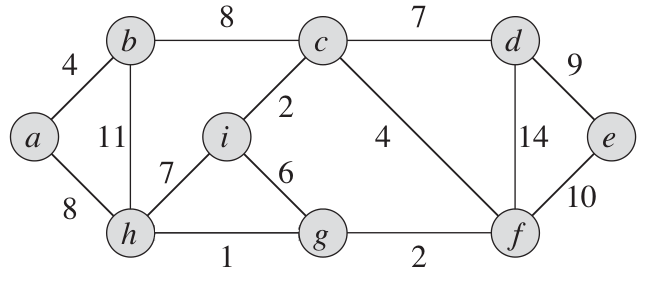
\includegraphics[width=80mm]{ej2aInicial.png}
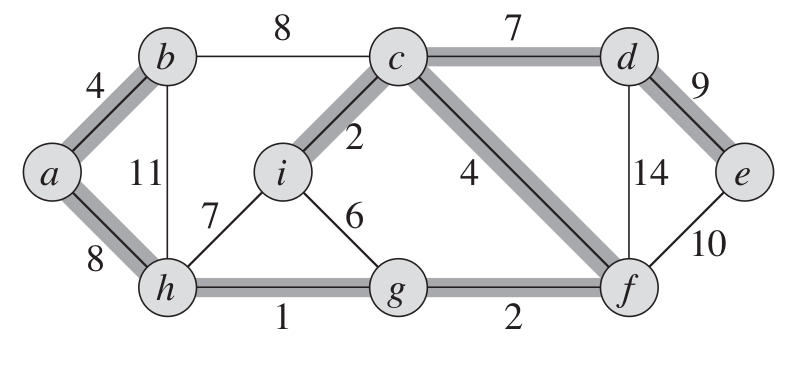
\includegraphics[width=80mm]{ej2aKruskal.png}
\caption{Comenzamos con el grafo incial (figura izquierda) y obtenemos el AGM utilizando Kruskal (figura derecha)}
\label{overflow}
\end{figure}  

\begin{figure}[H]
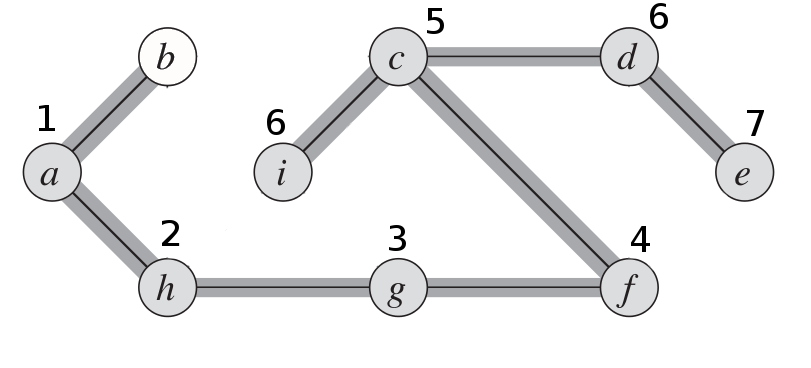
\includegraphics[width=80mm]{ej2aBFS1.png}
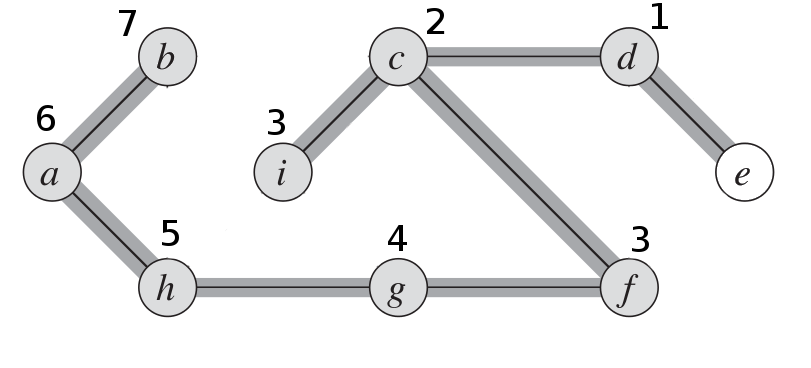
\includegraphics[width=80mm]{ej2aBFS2.png}
\caption{Aplicamos BFS desde un nodo arbitrario, en este caso b (figura izquierda) y luego lo aplicamos otra vez desde el nodo más lejano a b, en este caso e (figura derecha)}
\label{overflow}
\end{figure}  

\begin{figure}[H]
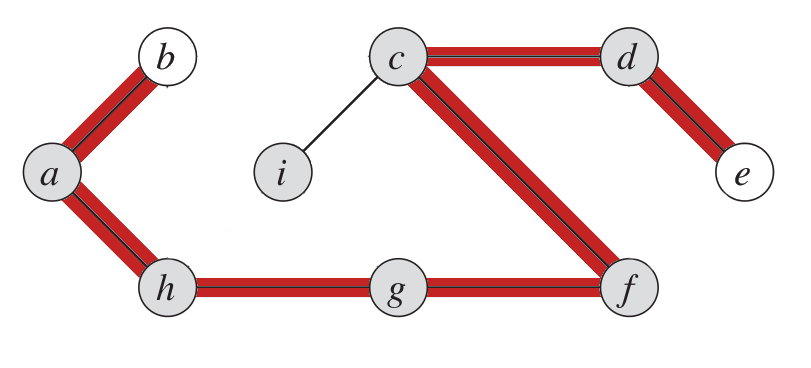
\includegraphics[width=80mm]{ej2aCMax.png}
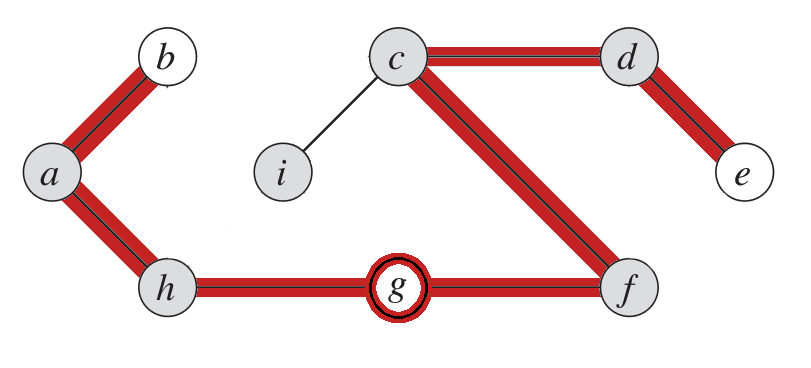
\includegraphics[width=80mm]{ej2aMaster.png}
\caption{Conseguimos el camino máximo (entre b y e) (figura izquierda) para después conseguir el nodo en la mitad del camino el cuál será el nodo master (figura derecha)}
\label{overflow}
\end{figure}  

\subsection{Solución (subproblema 1)}

Devolvemos un árbol generador mínimo del grafo que representa la red, obtenido utilizando el algoritmo de Kruskal.

El algoritmo de Kruskal fue implementado como se explica en el capítulo 21 de \textit{Introduction to Algorithms, 3rd Ed., Cormen, Leiserson, Rivest, Stein}, utilizando las heurísticas \textbf{union by rank} y \textbf{path compression}.


\subsubsection{Pseudocódigo}

\begin{pseudo}
  \Procedure{Enlaces-Costo-Mínimo}{$G = (V, E)$}
    \State $E' \leftarrow \textsc{Kruskal}(G)$                 \Ode{|E| \times log\, |V|}
    \PReturn $E'$
  \EndProcedure
\end{pseudo}


\subsection{Complejidad (subproblema 1)}

La complejidad total de la operación es $O(|E| \times log\, |V|)$. Como un grafo puede tener a lo sumo $|V|^2$ aristas, vale que $O(|E| \times log\, |V|) \subseteq O(|V|^2 \times log\, |V|)$. Recordando que nuestra red tenía $n$ servidores, reescribimos esta cota como $O(n^2 \times log\, n)$, que es estrictamente inferior a $O(n^3)$.


\subsection{Correctitud (subproblema 1)}

Veamos que lo que se nos pide se satisface con un árbol generador mínimo del grafo que representa la red servidores.

Para simplificar el análisis, supongamos que dados dos nodos $u$ y $v$ tales que existe un enlace entre ambos, $u$ transmite una copia del contenido a $v$ en el instante a continuación de haber recibido el contenido si y sólo si $v$ todavía no recibió una copia del contenido.

\newtheorem*{2a-arbol}{Teorema}
\begin{2a-arbol}
  Sea $G = (V, E)$ una instancia del problema y sea $u \in V$ un nodo que seleccionamos como master para el mecanismo de broadcast. Entonces el subgrafo $G'$ formado por $V$ y el subconjunto de enlaces $E' \subseteq E$ empleado para replicar el contenido desde $u$ al resto de los nodos es un árbol.
\end{2a-arbol}

\begin{proof}
  $G'$ es conexo, pues el mecanismo de broadcast alcanza todos los nodos del grafo, entonces existe un camino simple entre $u$ y el resto de los nodos en $V$. $G'$ no tiene ciclos, pues si los tuviera, algún nodo recibiría una copia del contenido más de una vez. Luego $G'$ es un árbol.
\end{proof}

\newtheorem*{2a-costo}{Teorema}
\begin{2a-costo}
  Sea $G = (V, E)$ una instancia del problema, sea $w: E \rightarrow \mathbb{N}$ la función de costo de los enlaces y sea $u \in V$. Entonces el costo de replicar el contenido desde $u$ al resto de los nodos por el mecanismo de broadcast es la suma del costo de los enlaces empleados $E' \subseteq E$, es decir $\sum_{i=1}^{|E'|} w(e_i)$.
\end{2a-costo}

\begin{proof}
  Cada nodo distinto del master recibe una copia del contenido una sola vez, es decir, se transmiten $|V| - 1$ copias de la información. Como $G$ es un árbol, éste tiene $|V| - 1$ aristas, y por cada una se transmite exactamente una de las $|V| - 1$ copias, pues en caso contrario al menos un nodo recibiría una copia del contenido más de una vez y al menos un nodo nunca recibiría su copia. Luego el costo total es la suma de transmitir exactamente una vez por cada enlace.
\end{proof}

Establecimos entonces que el subconjunto de enlaces usado por el mecanismo de broadcast forma un árbol y que el costo de esta operación es la suma de los costos de tales enlaces. 

Se nos pide hallar un subconjunto de enlaces para realizar broadcast a todos los nodos tal que el costo sea mínimo.

Es suficiente, pero no necesario, restringirnos a los subconjuntos de enlaces que forman árboles (un contraejemplo posible sería una red tal que todos sus enlaces tengan costo 0). Es decir, el conjunto de árboles generadores del grafo que representa la red, pues estos árboles necesariamente conectan todos los nodos del grafo.

Entonces un subconjunto de enlaces para realizar broadcast con costo mínimo, restringiéndonos al conjunto de árboles generadores del grafo que representa la red, es necesariamente un árbol generador mínimo.

Luego, basta con devolver cualquier árbol generador mínimo para satisfacer lo pedido.


\subsection{Solución (subproblema 2)}

Devolvemos el centro del árbol, es decir, un nodo tal que al tomarse como raíz, minimiza la altura del árbol.

A tal efecto, realizamos la siguiente serie de pasos:

\begin{itemize}
  \item Aplicamos el algoritmo BFS tomando como origen un nodo cualquiera y obtenemos el nodo más distante, al que llamamos $u$.
  \item Aplicamos el algoritmo BFS tomando como origen el nodo $u$ y obtenemos el nodo a mayor distancia de $u$, al que llamamos $v$.
  \item Obtenemos la secuencia de nodos que yacen el camino simple entre $u$ y $v$ (único, pues el grafo recibido como entrada del algoritmo es un árbol.)
  \item Devolvemos el nodo exactamente a la mitad del camino, redondeando para abajo si la cantidad de nodos es par.
\end{itemize}

El algoritmo BFS fue implementado como se explica en el capítulo 22 de \textit{Introduction to Algorithms, 3rd Ed., Cormen, Leiserson, Rivest, Stein}.

El procedimiento BFS usado a continuación toma un grafo $G = (V, E)$ y un vértice origen $s$ y devuelve un arreglo de distancias $d$ de dimensión $|V|$, tal que $d[i - 1] = \delta(s, v_i)$.

Notamos con $G.Ady(v)$ a la lista de adyacencia del vértice $v \in V$ en el grafo $G = (V, E)$.


\subsubsection{Pseudocódigo}

\begin{pseudo}
  \Procedure{Nodo-Master}{$G = (V, E)$}
    \State $d \leftarrow \textsc{BFS}(G, v_1)$                                         \Ode{|V| + |E|}
    \State $u \leftarrow$ nodo más distante a $v_1$ (recorremos todo el arreglo $d$)   \Ode{|V|}
    \State $d \leftarrow \textsc{BFS}(G, u)$                                           \Ode{|V| + |E|}
    \State $v \leftarrow$ nodo más distante a $u$ (recorremos todo el arreglo $d$)     \Ode{|V|}
    \State $c \leftarrow \textsc{Camino-Entre-Nodos}(G, u, v)$                         \Ode{|V|}
    \PReturn $c[|c|\; /\; 2]$                                                          \Ode{1}
  \EndProcedure

  \State

  \Procedure{Camino-Entre-Nodos}{$G = (V, E),\; u \in V,\; v \in V$}
    \State $d \leftarrow \textsc{BFS}(G, u)$                                           \Ode{|V| + |E|}
    \State $c \leftarrow \{ v \}$ \Comment{El camino a devolver}
    \State $w \leftarrow v$ \Comment{Nos paramos en el nodo $v$}
    \While{$w \neq u$} \Comment{Repetimos hasta llegar al nodo $u$}
      \For{$w'$ \In $G.Ady(w)$} \Comment{Recorremos la lista de adyacencia de $w$}
        \If{$d[w'] = d[w] - 1$} \Comment{Buscamos el siguiente nodo en dirección a $u$}
          \State $w = w'$
          \State $c \leftarrow c \cup \{ w \}$ \Comment{Agregamos el nodo hallado al final del camino}
          \Break
        \EndIf
      \EndFor
    \EndWhile
    \PReturn $c$
  \EndProcedure
\end{pseudo}


\subsubsection{Complejidad}

El procedimiento \textsc{Nodo-Master} realiza dos búsquedas BFS con costo $O(|V| + |E|)$. Luego invoca a \textsc{Camino-Entre-Nodos}, que a su vez realiza otra búsquda BFS con costo $O(|V| + |E|)$ y recorre un camino entre dos nodos del árbol. En el peor de los casos este camino incluye todos los nodos del árbol. Además, para cada nodo del camino se recorre su lista de adyacencia. Ahora bien, como se trata de un grafo no dirigido, una arista cualquiera aparece en las listas de adyacencia de ambos extremos. Como $G$ es un árbol, la cantidad de aristas es $|V| - 1$, y como en el peor caso se recorren las listas de adyacencia de todos los nodos, se recorren un total de $2 \times (|V| + 1)$ aristas, con una complejidad total de $O(|V| + 2 \times (|V| + 1)) = O(|V|)$.

La complejidad total del procedimiento es entonces $O(|V| + |E|) = O(|V| + |V| - 1) = O(|V|) = O(n)$.


\subsubsection{Correctitud}

Dado el AGM provisto por la ejecución de Kruskal, se busca probar que el procedimiento de encontrar el nodo \textit{master} es correcto.

Sean U y V dos nodos tales que las distancias entre ellos, l(U,V) , es máxima. Se puede ver que tomando R nodo que se encuentra en la mitad del camino entre U y V, la altura máxima del árbol considerado con R como raíz es l(U,V)/2. Si se seleccionara un vértice distinto de R, es fácil notar que se obtendría una altura mayor a l(U,V)/2.

Supongamos que elegimos como nodo maestro R. Sea l() la función de distancia entre dos nodos. La l(U,R) = l(U,V)/2 y l(R,V) $\leq$ l(U,V)/2. Si existiera otro nodo W, tal que l(R,W) > l(U,V)/2 tendríamos l(U,R) < l(R,W) y luego, debido a que solo hay un único camino entre dos nodos distintos en un árbol, tenemos que l(U,V) = l(U,R) + l(R,V) < l(U,R) + l(R,W) = l(U,W), l(U,V) < l(U,W) lo cuál contradice que l(U,V) tienen la mayor distancia. Por lo tanto, la profundidad, dado R como nodo maestro es l(U,V)/2. Ahora solo resta encontrar el camino máximo.

Debido que el algoritmo de BFS siempre termina en una hoja (si terminara en un nodo, habría una hoja más por la que seguir) y todo camino máximo tiene un extremo en una hoja (ya que si fuera un nodo su extremo, habría una hoja que sería camino más largo), se busca probar que la aplicación del algoritmo desde cualquier nodo arbitrario tendrá como nodo más distante un extremo del camino máximo en el árbol.

Dado un árbol AGM, el nodo arbitrario N1 elegido puede tener las siguientes ubicaciones:

\begin{itemize}
  \item Ser parte del camino máximo. Si esto ocurre, la hoja más lejana a N1 será trivialmente un extremo del camino máximo.
  \item No ser parte del camino máximo.
  
  Sea C1 el camino máximo del árbol de extremos U y V, y sea C2 el camino de longitud máxima entre N1 y N2, suponemos que N2 $\neq$ U, lo que implica que h(U) $<$ h(N2) (ya que, si N2 no es U, entonces N2 es un nodo con mayor distancia que U de N1), con h la altura del árbol tomando como raíz a N1. Llamamos también a X e Y las bifurcaciones de los caminos de N1 a U y a N2 respectivamente.

    \begin{figure}[ht!]
    \centering
    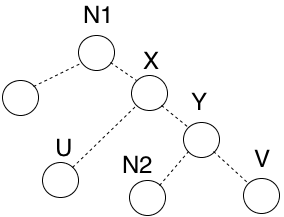
\includegraphics[width=60mm]{2b.png}
    \caption{Ejemplo gráfico de la suposición}
    \label{overflow}
    \end{figure}  

   Entonces, sea l función de longitud entre dos nodos, l(U,V) = h(U) + h(V) - 2*h(X) y l(U,N2) = h(U) + h(N2) - 2*h(X), y como h(N2) $>$ h(U) por ser N2 el nodo más lejano o de mayor altura, esto implica que l(U,N2) $>$ l(U,V) y esto es absurdo por ser C1 el camino máximo.
  
  Por el absurdo, concluimos que U = N2, es decir, que N2 es un extremo del camino máximo.
\end{itemize}

Al obtener un extremo del camino máximo, otra ejecución de BFS desde el extremo encontrado caerá sobre el caso trivial de pertenecer al camino máximo y encontrará el camino más lejano a este, su otro extremo.

Teniendo los dos extremos, buscamos el camino máximo del árbol (secuencia de nodos) mediante el procedimiento \textsc{Camino-Entre-Nodos}. Veamos que el procedimiento es correcto.

El procedimiento recibe el árbol $G = (V, E)$ y los extremos $u$ y $v$ de un camino simple de longitud máxima en $G$.

Como $G$ es un árbol, el camino simple entre $u$ y un nodo $w$ cualquiera es único. Si tomamos como raíz del árbol al nodo $u$, el único camino simple posible desde $w$ a $u$ lo realizamos moviéndonos hacia el nodo antecesor a $w$, y repitiendo hasta alcanzar $u$. Veamos que el procedimiento hace exactamente eso, partiendo del nodo $v$.

El procedimiento aplica el algoritmo BFS sobre $G$ tomando como origen el vértice $u$, de manera de computar las distancias entre $u$ y el resto de los vértices en $V$ (distancia medida en cantidad de aristas.) Luego se para en $v$, busca su nodo adyacente de distancia $\delta(v) - 1$ (es decir su antecesor), y repite la operación hasta alcanzar el nodo $u$. Luego, el procedimiento cumple con lo dicho en el párrafo anterior.

Tras cada paso, el procedimiento guarda el vértice visitado en la lista de vértices del camino entre $u$ y $v$. Es decir, el procedimiento recorre la secuencia de antecesores de $v$ hasta llegar al nodo raíz $u$. Finalmente devuelve la secuencia obtenida, que necesariamente es la secuencia de vértices que yacen en el camino simple entre $u$ y $v$.

Una vez obtenido el camino, el nodo que se encuentre en la mitad de este, será el nodo master.


\subsection{Preguntas adicionales}

Mostrar con un contraejemplo que es posible resolver las dos partes por separado de manera óptima pero que aún así haya una solución en la que la replicación termine en menos tiempo. Comentarposibles soluciones al problema.


¿Cómo se debe modificar la solución si en lugar de transmitir por broadcast se lo hace por
multicast ,es decir, se debe mandar un paquete a cada destino, sin hacer copias?


\subsection{Experimentos computacionales}


\subsubsection{Caso general}

\begin{figure}[H]
  \centering
  \dosgraficos{problema2-caso-general}
              {problema2-caso-general-n}
  \caption{Caso general}
\end{figure}


\subsubsection{Instancias aleatorias}

\begin{figure}[H]
  \centering
  \dosgraficos{problema2-instancias-aleatorias}
              {problema2-instancias-aleatorias-n}
  \caption{Instancias aleatorias}
\end{figure}



%%%%%%%%%%%%%%%%%%%%%%%%%%%%%%%%%%%%%%%%%%%%%%%%%%%%%%%%%%%%%%%%%%%%%%%%%%%%%%%
%% Problema 3: Transportes pesados                                           %%
%%%%%%%%%%%%%%%%%%%%%%%%%%%%%%%%%%%%%%%%%%%%%%%%%%%%%%%%%%%%%%%%%%%%%%%%%%%%%%%


\newpage

\section{Problema 3: Transportes pesados}

Una empresa que fabrica ladrillos tiene sus fábricas en varios puntos de una provincia. La misma se encarga de transportar los ladrillos a los clientes que están distribuísdos en distintas ciudades de la provincia.\\
Como las rutas de esta provincia no están preparadas para soportar el paso de los camiones, la empresa tiene que fortalecer las rutas para que puedan ser utilizadas por los camiones.\\
Dado que cada ruta tiene un costo de inversión proporcional a la longitud de la misma, se pide replanificar las rutas habituales de manera tal de minimizar los gastos que implicará el fortalecimiento de las rutas para que cada cliente pueda ser provisto desde al menos una fábrica.\\
La complejidad temporal del \textbf{peor caso} deberá ser \textbf{O($C^2$)} o bien \textbf{O(R$log$(C)).}

\textbf{Ejemplos del problema y sus soluciones:}

\textbf{Entrada}: 2 fábricas, 2 clientes y 4 rutas.
\begin{itemize}
\item{La lonitud de la ruta desde la fábrica 1 a la fábrica 2 es 1.}
\item{La lonitud de la ruta desde la fábrica 1 al cliente 1 es 4.}
\item{La lonitud de la ruta desde la fábrica 2 al cleinte 2 es 5.}
\item{La lonitud de la ruta desde el cliente 1 al cliente 2 es 7.}
\end{itemize}

\begin{figure}[H]
\centering
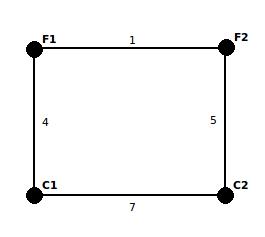
\includegraphics[width=60mm]{../ejemplo_graficos/CosoDosSubconjuntos.png}
\caption{Grafo inicial}
\label{1}
\end{figure} 

\begin{figure}[H]
\centering
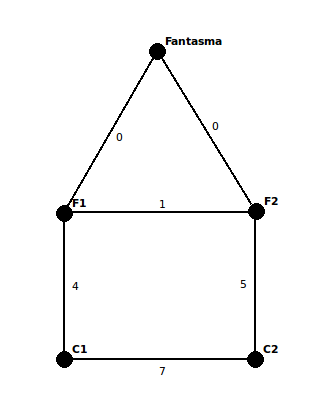
\includegraphics[width=60mm]{../ejemplo_graficos/CosoDosSubconjuntosConNodoFantasma.png}
\caption{Se le agrega el nodo \textit{fantasma}}
\label{2}
\end{figure} 

\begin{figure}[H]
\centering
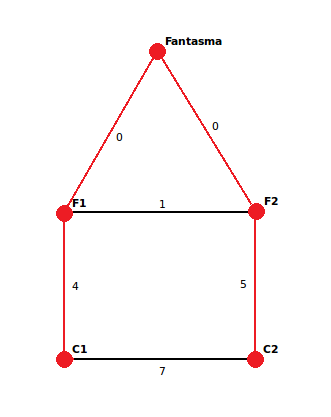
\includegraphics[width=60mm]{../ejemplo_graficos/CosoDosSubconjuntosConNodoFantasmaSolucion.png}
\caption{AGM con nodo \textit{fantasma}}
\label{3}
\end{figure} 

\begin{figure}[H]
\centering
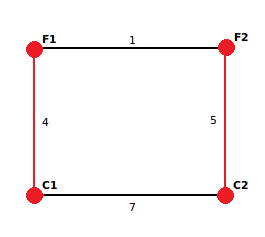
\includegraphics[width=60mm]{../ejemplo_graficos/CosoDosSubconjuntosSolucion.png}
\caption{Se le quita el nodo \textit{fantasma}}
\label{4}
\end{figure} 

\begin{figure}[H]
\centering
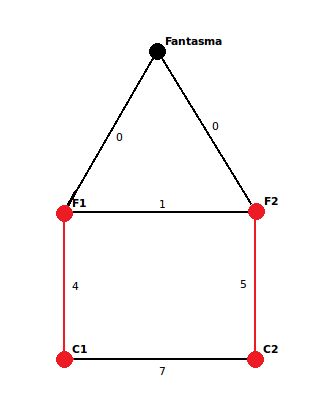
\includegraphics[width=60mm]{../ejemplo_graficos/CosoDosSubconjuntosSolucionSinFantasma.png}
\caption{Solución final}
\label{5}
\end{figure} 

\textbf{Salida}: Costo total de inversión 9. Las rutas utilizadas fueron:
\begin{itemize}
\item{de la fábrica 1 al cliente 1.}
\item{de la fábrica 2 al cliente 2.}
\end{itemize}

\subsection{Solución}

Dada una serie de aristas y sus respectivos costos, que representan las rutas entre clientes y fábricas y el costo de pavimentación, utilizamos para la resolución una modificación del conjuto de datos para luego aplicar el algoritmo de Kruskal con la estrucuta Disjoint-Set.

La idea de la utilización del algoritmo de Kruskal nace de la necesidad de conseguir un bosque de AGM's entre clientes y fábricas, lo que nos permitirá conseguir los caminos que los interconecten de mínimo costo. Como en nuestro caso, solo se necesita que una fábrica este conectada por una serie de rutas a otros clientes, creamos un nodo \textit{fantasma} al cuál le conectamos cada fábrica mediante una arista de costo cero para poder tener un único set que forzará a que el algoritmo solo conecte una única vez una fábrica con cada set disjunto.

El resultado obtenido será un árbol AGM al cual, al sacarle el nodo \textit{fantasma} y las aristas de las fábricas a este, como solo se unían los set disjuntos con una sola fábrica, se forma un bósque, donde los árboles de este tendran las rutas necesarias para pavimentar y minimizar el costo de inversión.

\subsubsection{Pseudocódigo}
\begin{pseudo}

\State ranking : vector de enteros

\State $tupla <nodo1 : entero, nodo2 : entero, costo : entero>$ es $ruta$
\Procedure{problema3}{nodos : entero, cantFabricas : entero, rutas : vector de ruta}
	\For{i=0 To Tamaño(parent)} parent[i] = i \EndFor						\Ode{C}
	\For{i=0 To Tamaño(ranking)} ranking[i] = 0 \EndFor						\Ode{C}

    \State camino\_minimo : vector de ruta									\Ode{1}
    \For{unsigned i = 0; i < cantFabricas; ++i}								\Ode{1}
        \State rutas.Agregar(ruta(i, nodos, 0))								\Ode{1}
    \EndFor

	

    \State Ordenar(rutas) ordenar de manera creciente las rutas por costo \Ode{R log R}

    \For{i = 0 To Tamaño(rutas)}
        \State set1 : entero = Find(nodo1(rutas[i]))						\Ode{1}
        \State set2 : entero = Find(nodo2(rutas[i]))						\Ode{1}
        \If{set1 != set2}													\Ode{1}
            \State Make\_union(set1, set2)									\Ode{1}
            \State camino\_minimo.Agregar(rutas[i])							\Ode{1}
        \EndIf    
    \EndFor

	 

    \State res : vector de rutas de tamaño (camino\_minimo.size() - cantFabricas)   \Ode{C}
    \For{i = cantFabricas To Tamaño(camino\_minimo)}
        \State res.Agregar(ruta(nodo1(camino\_minimo[i]), nodo2(camino\_minimo[i]), costo(camino\_minimo[i])))	\Ode{1}
    \EndFor
    \Return res
\EndProcedure

\end{pseudo}

\subsection{Complejidad}

Como se agrega un conjunto nuevo de aristas acotado por la cantidad de fábricas, se obtiene un costo de O(F) para crear las nuevas rutas que se conectarán al nodo \textit{fantasma}. Como R $>$ F, O(F) $\in$ O(R) acotando la cantidad de rutas a O(R).

Debido a que para el ordenamiento de las rutas, utilizamos la función Sort() de la STL de C++, se obtiene una costo de O(R * log R), siendo R rutas, lo que equivale a O(R * log $(C+F)^2$), siendo C clientes y F fábricas por ser C+F la mayor cantidad de aristas posibles. Por ser F menor que C, O(F) $\subset$ O(C), log($(C+F)^2$) $\subset$ log($C^2$). Siendo O($C^2$) la cota superior para la cantidad de aristas, la complejidad equivale a O(R * 2 log C) $\subset$ O(R * log C).

Como se utiliza el algoritmo de Kruskal, al igual que en el segundo problema, la complejidad de obtener los subconjuntos de rutas que unen clientes con fábricas es de O(R).

Como O(R) $\subset$ O(R * log C), la complejidad final del algoritmo es O(R * log C).
\subsection{Correctitud}
Un bosque con aristas de peso mínimo y una sola conexión a una fábrica para cada árbol, es una solución correcta, ya que, para todo árbol del bosque, sus nodos (clientes) y única fábrica (ya que más de una necesitaría otra ruta y no sería mínimo), estan conectados mediante las aristas de menor costo de pavimentación, haciendo que el costo sea mínimo.

Para demostrar la correctitud del algoritmo, debemos demostrar que Kruskal aplicado a la modificación realizada a nuestro conjunto de datos devuelve un AGM al que, al podarle el nodo \textit{fantasma} se convierte en un bosque de árboles, cada uno con clientes y una fábrica asociada conectados con costo mínimo.

Debido a que asumimos que los costos de pavimentación de todas las rutas son mayor a 0 (ya que el costo es proporcional a la longitud), en las primeras iteraciones (exactamente \#(F)) del algoritmo, se unirán todas las fábricas en único set. Por esta unión, Kruskal se encargará de unir una única vez una fábrica con los conjuntos de clientes. En las próximas iteraciones de Kruskal, el algoritmo se comportará  de la manera habitual.

Dada la solución obtenida por Kruskal, queremos ver que al podar el nodo fantasma y sus aristas, el bosque generado es mínimo.

Por el absurdo. Supongo que la solución obtenida no es óptima, esto implica que existe otro bosque solución el cuál tiene un costo menor. Para este bosque conecto sus fábricas con un nodo \textit{fantasma} y como los pesos de las aristas agregadas para conectar el nodo fantasma son 0, el árbol generado es AGM. Absurdo, ya que el árbol original devuelto por Kruskal ya era AGM.

Podemos concluir, por el absurdo que el bosque solución obtenido es el ópitmo en costo.


\subsection{Experimentos computacionales}


\newpage


\subsubsection{Peor caso}

\begin{figure}[H]
  \centering
  \tresgraficos{problema3-peor-caso}
               {problema3-peor-caso-logn}
               {problema3-peor-caso-n}
  \caption{Peor caso}
\end{figure}


\subsubsection{Mejor caso}

\begin{figure}[H]
  \centering
  \tresgraficos{problema3-mejor-caso}
               {problema3-mejor-caso-logn}
               {problema3-mejor-caso-n}
  \caption{Mejor caso}
\end{figure}


\subsubsection{Instancias aleatorias}

\begin{figure}[H]
  \centering
  \tresgraficos{problema3-instancias-aleatorias}
               {problema3-instancias-aleatorias-logn}
               {problema3-instancias-aleatorias-n}
  \caption{Instancias aleatorias}
\end{figure}


%%%%%%%%%%%%%%%%%%%%%%%%%%%%%%%%%%%%%%%%%%%%%%%%%%%%%%%%%%%%%%%%%%%%%%%%%%%%%%%
%% Conclusiones                                                              %%
%%%%%%%%%%%%%%%%%%%%%%%%%%%%%%%%%%%%%%%%%%%%%%%%%%%%%%%%%%%%%%%%%%%%%%%%%%%%%%%


\newpage

\section{Conclusiones}




%%%%%%%%%%%%%%%%%%%%%%%%%%%%%%%%%%%%%%%%%%%%%%%%%%%%%%%%%%%%%%%%%%%%%%%%%%%%%%%
%% Código fuente para el problema 1                                          %%
%%%%%%%%%%%%%%%%%%%%%%%%%%%%%%%%%%%%%%%%%%%%%%%%%%%%%%%%%%%%%%%%%%%%%%%%%%%%%%%


\newpage

\begin{appendices}

\section{Código fuente para el problema 1}


\subsection{problema1.h}

\subsection{problema1.cpp}




%%%%%%%%%%%%%%%%%%%%%%%%%%%%%%%%%%%%%%%%%%%%%%%%%%%%%%%%%%%%%%%%%%%%%%%%%%%%%%%
%% Código fuente para el problema 2                                          %%
%%%%%%%%%%%%%%%%%%%%%%%%%%%%%%%%%%%%%%%%%%%%%%%%%%%%%%%%%%%%%%%%%%%%%%%%%%%%%%%


\newpage

\section{Código fuente para el problema 2}


\subsection{problema2.h}

\subsection{problema2.cpp}



%%%%%%%%%%%%%%%%%%%%%%%%%%%%%%%%%%%%%%%%%%%%%%%%%%%%%%%%%%%%%%%%%%%%%%%%%%%%%%%
%% Código fuente para el problema 3                                          %%
%%%%%%%%%%%%%%%%%%%%%%%%%%%%%%%%%%%%%%%%%%%%%%%%%%%%%%%%%%%%%%%%%%%%%%%%%%%%%%%


\newpage

\section{Código fuente para el problema 3}


\subsection{problema3.h}

\subsection{problema3.cpp}


\end{appendices}

\end{document}